\chapter{A Privacy-preserving Framework for IoT Devices}

In this chapter, we present our primary contribution: a privacy-preserving framework for generalized IoT devices. We propose communication and attacker models and state security and usability features of the framework.

\section{Communication models}

In this thesis, we consider only one communication model. In our model, the IoT devices interact with end-user devices (e.g., smartphones). The end-user devices have direct access and can remotely control the IoT device.

It is worth mentioning that there exists another communication model for IoT systems. IoT devices sometimes need to communicate with each other to enable automatic workflows. However, we consider the first model to be primary in IoT systems and focus on it. We briefly discuss the IoT-to-IoT scenario in Chapter 5. 

\textit{Fig. \ref{fig:cm1}} and \textit{Fig. \ref{fig:cm2}} show the idea of the two communication models we discussed above. 



\begin{figure}
	\centering
		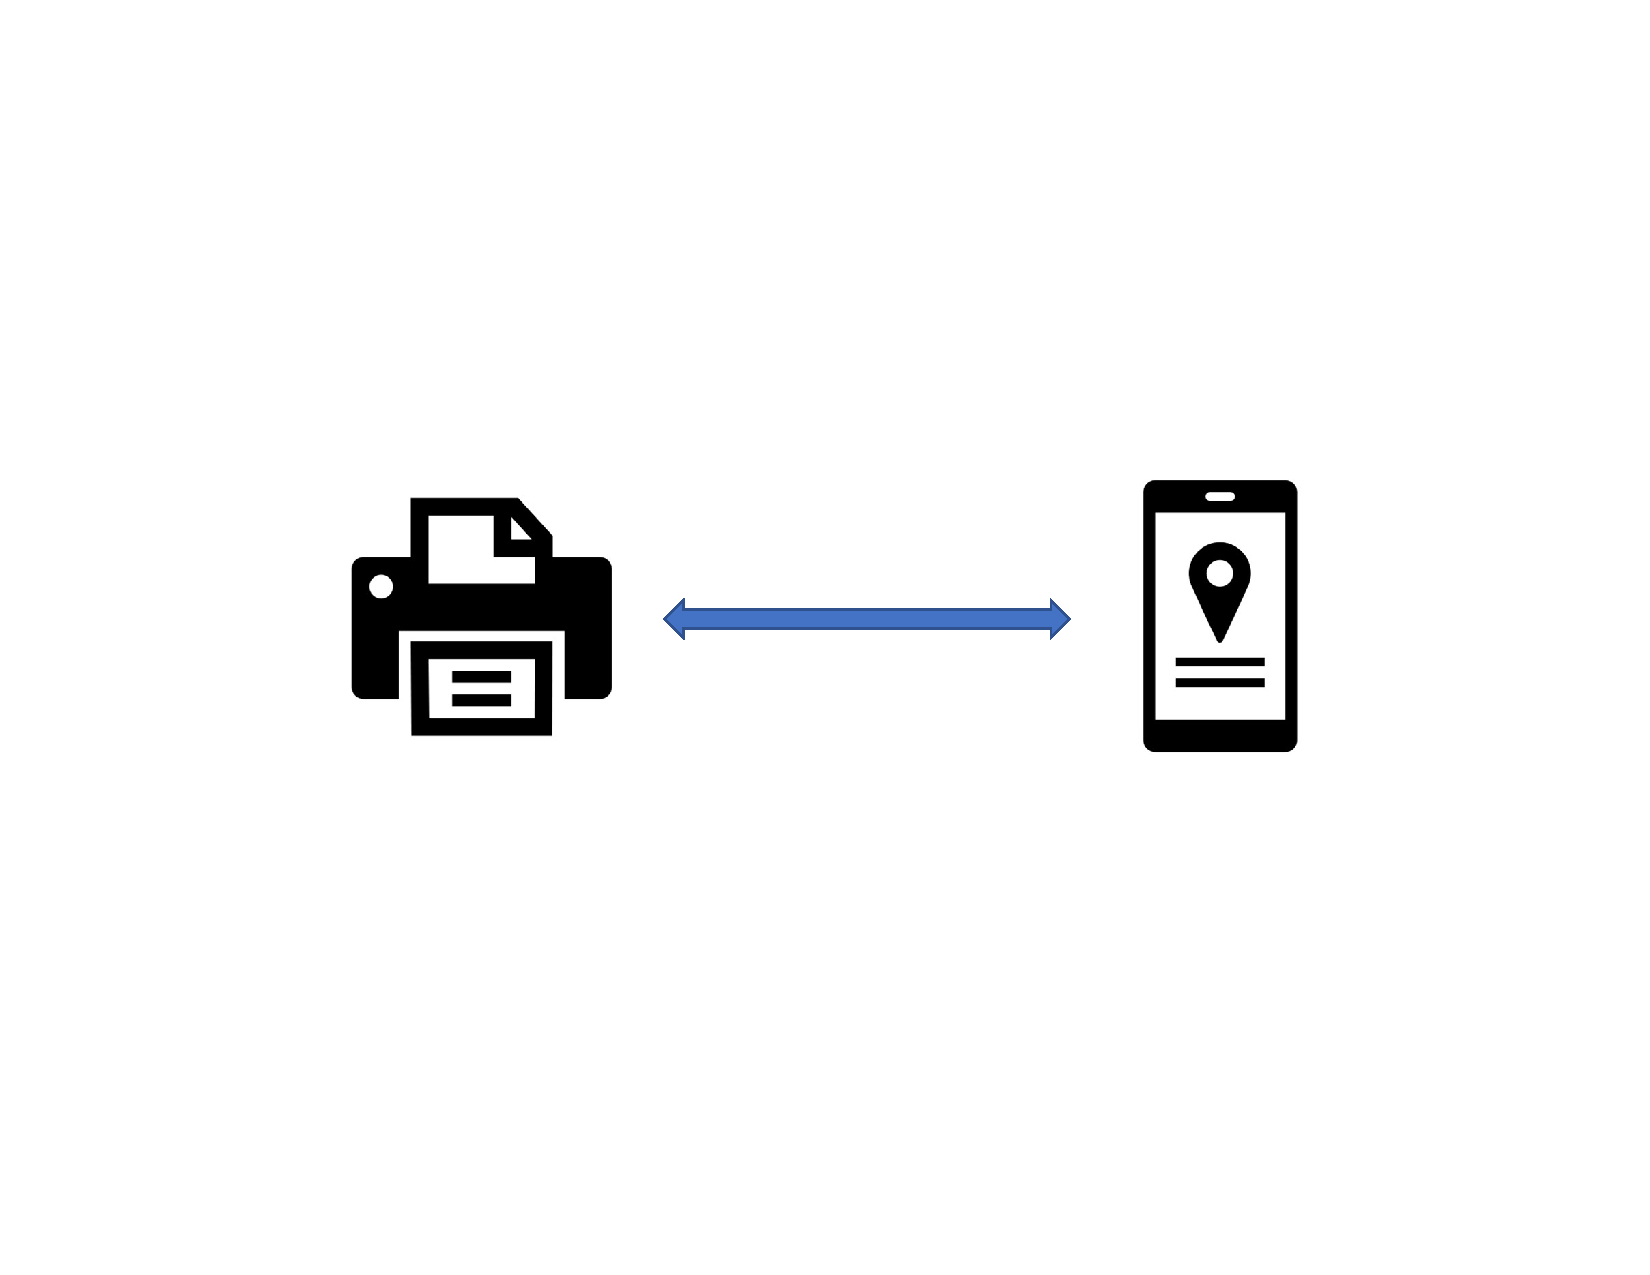
\includegraphics[width=0.6\linewidth]{comm_model_1.pdf}
		\caption{Communication model: IoT-user}
		\label{fig:cm1}
\end{figure}
\begin{figure}
	\centering
		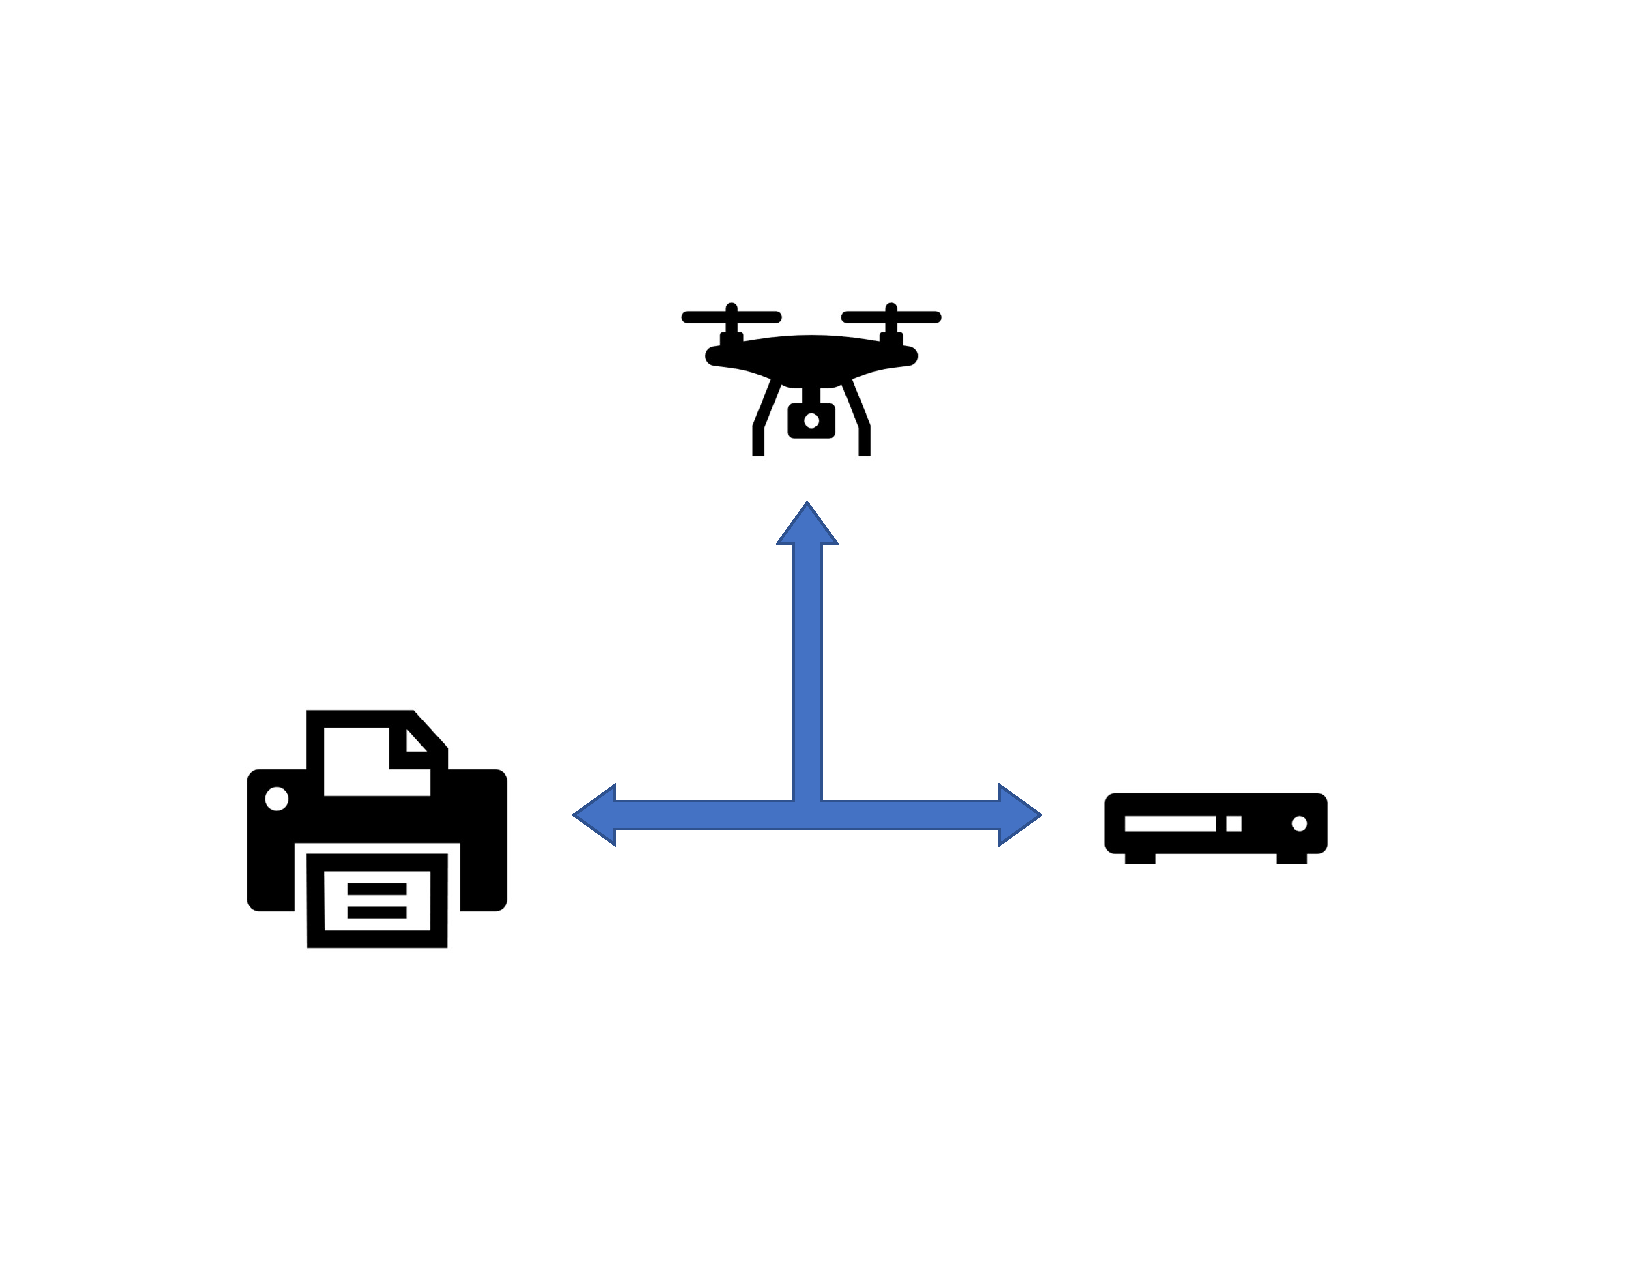
\includegraphics[width=0.6\linewidth]{comm_model_2.pdf}
		\caption{Communication model: IoT-IoT}
		\label{fig:cm2}
\end{figure}

\section{Threat model}

Our analysis assumes an active network threat model where attackers are located both inside and outside the home network. The attackers may have capabilities similar to or the same as an ISP

Traditionally, IoT devices run globally searchable services \cite{antonakakis2017understanding}. Consequently, IoT devices are exposed to potential vulnerabilities and attacks. Attackers can discover potentially vulnerable devices by discovering them through IoT search engines (e.g., Shodan) or using whole-Internet scanning tools (e.g., ZMAP \cite{wiemer2001software}).

Furthermore, mobile devices running paired service applications with home IoT devices usually access the Internet via untrusted networks, cellular networks, or free Wi-Fi hotspots. In such cases, on-path attackers can capture and inspect data packets, retrieve sensitive data or even locate and attack the communication's endpoints. 

In the following, we discuss potential attackers, their capabilities, and our system's security guarantees.

\subsection{Actors and capabilities}
We consider the following two types of adversaries:

\textbf{In-network adversaries} are adversaries who have access to the users' home network. Such adversaries may eavesdrop and identify traffic from particular devices in the user's home, including the IoT device and router.


\textbf{Out of network but on-path adversaries} are adversaries located outside the user's home network (and have no access to it). Such adversaries cannot differentiate between devices in the network but can eavesdrop, analyze, and modify the user’s traffic in aggregate. 

Furthermore, the adversary can obtain and analyze IoT devices and client devices. They may inspect programs and source code and use their copy of client apps to attempt to access the user's device.

\textbf{Service adversaries} are adversaries running third-party services (e.g., push notification services) adopted by the IoT system. Such operators should not be able to enumerate all IoT users or know when all events occurred.

They may have access to the system's adapted push notification service, which means they can eavesdrop and/or modify the packets or send packets to the user's phone at will.
\subsection{Security and privacy guarantees}

Our framework offers the following security and privacy guarantees:

\begin{itemize}
	\item \textbf{Strong authentication}. The device should only be accessible to authorized clients. \textit{Out-of-network adversaries} should not have access to the data (including the history of usage and data captures by the sensor) regardless of the measurements they take.
	\item \textbf{Anonymity on both sides}. The communication between the client and home IoT device should be anonymized. \textit{Out-of-network adversaries} should get identical information (including IP address and physical address) of neither the client nor IoT device.
	\item \textbf{End-to-end security}. The traffic between the client and home IoT devices should be end-to-end encrypted. Neither \textit{In-network adversaries} nor \textit{Out-of-network adversaries} should be able to read the content in the packets transmitted.
	\item \textbf{Attack resistance}. The attack surface against the IoT devices should be small (e.g., resists DoS attacks).
	\item \textbf{Resistance to traffic analysis}. \textit{Out-of-network adversaries} and \textit{Service adversaries} should not be able to obtain the user's sensitive information (including but not limited to use history of the IoT device, time of events) by analyzing the encrypted traffic.
\end{itemize}

\section{Features}
In addition to the security guarantees, the system should have  usability features:

\begin{itemize}
	\item \textbf{Access from end-user devices.} The system should be accessible from an end-user device. The user should be able to control and retrieve data from the device remotely. 
	\item \textbf{Support for NAT-piercing and dynamic IP.}  For compatibility with typical home networks, the system should work on devices located behind firewalls, gateway routers or are otherwise normally inaccessible from the outside Internet. Similarly, our framework do not assume static IPs and is compatible with home networks with dynamic IP addresses.
	\item \textbf{Decentralization.} Critically, the system should try to avoid all points of decentralization. The user should not register to third-party services or external websites to have the service running or retrieving data. This eliminates centralization of data, and thus protects users' sensitive information.
	\item \textbf{Real-time data transmission.} The system should let its user retrieve data in real-time and send notifications to the end-user device (e.g., a smartphone) whenever the IOT devices wishes to alert the users.
\end{itemize}



\section{Constructing a privacy-preserving framework for IoT devices.}
To achieve the security guarantees described above, we introduce the Tor network in the communication between home IoT devices and end-user devices. The Tor network, a common approach for achieving anonymity\cite{dingledine2004tor}, has the following features, which makes it a good choice for privacy-preserving systems:


\subsection{Achieving strong authentication and end-to-end confidentiality.} This task is non-trivial since IoT devices have limited interfaces. The framework tackles this by enabling a pairing phase in which smartphone devices can pair with the IoT device and exchange key material. The pairing phase must be manually initiated on the IoT device, and should be resistant to man-in-the-middle attacks. One instantiation of this (see next Chapter) is to have the IoT device set up an mDNS service, which makes it possible for a smartphone in the same network to connect to share key material. Once key material is shared, all data sent and received by both the IoT device and the smartphone application should be end-to-end encrypted using standard protocols (e.g., TLS). Additional methods for enabling strong authentication are described below (see "Attack resistance").

\subsection{Resistance to traffic analysis.} A key feature of the framework is that it (1) obscures the use of the IoT device and (2) provides resistance to traffic analysis from potential on-path adversaries. Both are achieved by tunneling all traffic from the IoT device through an anonymity network, such as Tor. Additionally, covertness can be achieved by using Tor pluggable transports \cite{shahbar2015traffic}, which further conceal the anonymity network's use. This makes it difficult for an adversary to even identify that the monitored user's home network contains the IoT device, given that Tor has a wide variety of uses well beyond obscuring IoT traffic.

Push notification services present another opportunity for traffic analysis. In traditional IoT systems, the IoT device sends a push notification through an operator (e.g., Google on Android and Apple on iOS) in order to alert the owner of the device. This allows the push notification operator to learn (1) the users who have the IoT device (by virtue of forwarding the alerts to their smartphones), (2) when such alerts occurred, and (3) if not encrypted, the contents of the notification. We protect against all three forms of information leakage by avoiding centralized push notification services, and instead, sending push notifications directly (or more precisely, through Tor) from the IoT device to the smartphone. In the next Chapter, we show that the power and data cost of such an operation are surprisingly small.

\subsection{Attack resistance.} Our framework requires the IoT device to operate as a Tor onion service (previously called \textit{hidden services}). Onion services are only accessible via the Tor network. This provides strong resistance to denial-of-service attacks, since Tor does not support voluminous amounts of traffic (since it is slow) as all traffic must traverse a series of (unfortunately overloaded) relays. Additionally, the use of hidden services also further supports strong authentication, since onion services optionally support authentication -- meaning that the service is only accessible to clients who possess the correct keys.

\subsection{Resistance to enumeration.} The use of onion services also provides resistance to enumeration. Traditional IoT devices may be (and often are) discoverable on the Internet, and indeed, search engines such as Shodan \cite{matherly2015complete} provide queryable interfaces for identifying particular IoT devices. This poses a significant security threat, since a single vulnerability in an IoT device could easily be used as a mechanism to construct a (potentially large) botnet. Our framework resists such enumeration through the use of onion services. Onion services cannot be easily enumerated \cite{winter2018tor} \cite{chaabane2010digging} since connecting to them requires knowledge of both the .onion URL and, in our case, the credentials for accessing the onion service.